\documentclass{LTHthesis}
%\documentclass[svenska]{LTHthesis} % Use this line instead if the thesis is written in Swedish.
\usepackage[T1]{fontenc}
\usepackage[utf8]{inputenc}
\usepackage{mathptmx, helvet}
\usepackage{graphicx}
\graphicspath{{figures/}}

\addbibresource{references.bib}

% Marks text that is still to be written. Search for \TODO before submission.
\newcommand{\TODO}[1]{\textbf{[TODO: #1]}}

\begin{document}
\begin{titlepages}
\author{Otto M\"orner}
\title{An LLM as an Offline Heuristic Learner\\ for Interpretable Supervisory\\ Process Control} % Working title
\year{2026}      % TODO: year of submission
\month{\TODO{month}}
\TFRT{9999}      % You will get the number from the department.
\printer{Media-Tryck}  % Probably. You may get other information from the department.
\end{titlepages}

\chapter*{Abstract}
% Draft abstract based on the toy-example results; revise once the industrial
% comparison is done.
Advanced process controllers based on learned models, such as TD-MPC, can
perform well but are hard to inspect, verify and audit. This thesis
investigates an alternative in which a large language model (LLM) is used
\emph{offline} as a meta-supervisor: it reads logs, scores and decision
traces from a simulated process and writes a small, deterministic supervisory
function in Python. The function runs on top of fixed PID loops, raises
per-loop anomaly flags and adjusts setpoints. Every candidate passes a static
security check and a sandboxed evaluation on a battery of fault scenarios, and
is only promoted if it improves on the current champion without regressing
any single scenario.

The approach is developed on three toy processes of increasing difficulty: a
single leaking tank, a two-tank cascade, and the quadruple-tank process. On
all three, the generated supervisors reduced the score on the development
scenarios by 72--96\% compared with PID control alone. On the quadruple-tank process, supervisors
generated with LLM reasoning enabled matched a perfect-detection oracle on
both the development and the held-out scenarios within two to three
generations, whereas the same search without reasoning stagnated at about
4.5 times the oracle score. The experiments also show that the design of the
evaluation, including safeguards against specification gaming and checks that
the test bed itself is sound, matters as much as the choice of model.
\TODO{Add the result of the comparison on the industrial process and against TD-MPC.}


\chapter*{Acknowledgements}
\TODO{Thank the supervisors at Weir and at the Department of Automatic Control, the examiner, and others who helped.}

\tableofcontents

\chapter{Introduction}
\label{ch:introduction}

\section{Motivation}
Mineral processing circuits such as grinding mills are multivariable, strongly
coupled and subject to frequent disturbances \cite{pomerleau2000}. They are
typically run with decentralized PID loops at the base layer and a supervisory
layer on top that coordinates setpoints and handles abnormal situations.
Learned controllers such as TD-MPC \cite{hansen2022tdmpc,hansen2024tdmpc2}
can perform well in this role, but their behaviour is encoded in neural
networks, which makes it hard for engineers to inspect, verify and certify
what the controller will do in situations it has not seen.
\TODO{Describe the industrial setting at Weir: the process, the current TD-MPC controller and why interpretability and auditability matter there.}

Recent work has shown that large language models (LLMs) can act as the
mutation operator in an evolutionary search over \emph{programs}, with an
automated evaluator as the only judge of quality
\cite{romeraparedes2024funsearch,novikov2025alphaevolve,ma2024eureka,weng2026lbg}.
The result of such a search is ordinary source code that can be read,
reviewed and tested like any other code. This thesis asks whether that idea
can produce supervisory control logic of practical quality.

\section{Research questions}
\begin{enumerate}
\item Can an LLM, used offline as a heuristic learner, generate deterministic,
  security-checked supervisory control code that performs close to a learned
  controller such as TD-MPC while remaining interpretable?
\item What information does the LLM need about the process, the evaluation and
  earlier attempts to make steady progress?
\item How must the evaluation be designed so that the search improves the
  intended behaviour rather than exploiting the score?
\item How much LLM reasoning is needed, and what does it cost?
\end{enumerate}
\TODO{Refine the research questions together with the supervisors.}

\section{Approach and contributions}
The work uses a three-layer architecture (Chapter~\ref{ch:method}): fixed PID
loops at the bottom, a deterministic supervisor function in the middle, and an
offline LLM-driven learner at the top that rewrites the supervisor between
runs. The approach is developed and evaluated on three toy processes of
increasing difficulty (Chapter~\ref{ch:toy}) before it is applied to the
industrial process. The contributions so far are:
\begin{itemize}
\item an implementation of the three-layer architecture with a security
  sandbox for generated code and a scoring scheme with safeguards against
  specification gaming;
\item results on a single tank, a two-tank cascade and the quadruple-tank
  process, including a comparison with a perfect-detection oracle;
\item an ablation of the LLM's reasoning effort on the quadruple-tank process.
\end{itemize}
\TODO{Add the industrial case study and the comparison with TD-MPC.}

\section{Outline}
Chapter~\ref{ch:background} gives background on supervisory process control,
fault detection and LLM-guided program search. Chapter~\ref{ch:method}
describes the architecture, the security sandbox, the scoring and the training
loop. Chapter~\ref{ch:toy} presents the three toy examples and their results.
Chapter~\ref{ch:discussion} discusses the findings and their limitations, and
Chapter~\ref{ch:conclusions} concludes.

\chapter{Background}
\label{ch:background}

\section{Supervisory process control}
Industrial processes are usually controlled hierarchically. Fast PID loops at
the base layer keep individual variables at their setpoints, while a slower
supervisory layer chooses those setpoints, coordinates interacting loops and
reacts to abnormal situations \cite{astrom2011,pomerleau2000}. In a
multivariable process, the pairing of manipulated and controlled variables
in the base layer matters: the relative gain array \cite{bristol1966} shows
whether a decentralized pairing will work with or against the process
interactions.
\TODO{Expand with the supervisory structure used in grinding circuits and at Weir.}

\section{Fault detection}
A supervisor must decide from measurements alone whether a fault is present.
Model-based fault detection compares measured behaviour with what a process
model predicts for the fault-free case and raises an alarm when the residual
is large enough \cite{isermann2006}. The trade-off between missed detections,
false alarms and detection delay is central, and it is reflected directly in
the scoring used in this thesis (Section~\ref{sec:scoring}).
\TODO{Expand with residual generation and evaluation, and threshold selection.}

\section{LLM-guided program search}
FunSearch \cite{romeraparedes2024funsearch} pairs an LLM with an automated
evaluator in an evolutionary loop: the LLM proposes programs, the evaluator
scores them, and the best programs are used as context for new proposals.
AlphaEvolve \cite{novikov2025alphaevolve} scales the same idea into a general
coding agent and reports that removing the rich problem context from the
prompt is among the most harmful ablations. Eureka \cite{ma2024eureka} uses an
LLM to write reward functions for reinforcement learning and feeds numeric
results back in a reflection step. \textcite{weng2026lbg} describes an
iterative workflow in which a policy is improved by inspecting execution
traces and rewriting code instead of through gradient updates. This thesis applies the
pattern to supervisory control, where the evaluator is a closed-loop
simulation with fault injection.

\section{Learned controllers}
TD-MPC \cite{hansen2022tdmpc} and TD-MPC2 \cite{hansen2024tdmpc2} learn a
latent world model, plan over a short horizon in that model and bootstrap
long-horizon value with temporal-difference learning. They are the learned,
black-box side of the comparison in this thesis.
\TODO{Summarize what TD-MPC can do that a readable rule set cannot, and vice versa.}

\section{Specification gaming}
An optimizer that is scored by a metric will exploit weaknesses in that
metric \cite{amodei2016,krakovna2020}. LLM-guided search is no exception: in
this work, candidates repeatedly found ways to improve the average score
while behaving worse, which motivated the safeguards in
Section~\ref{sec:scoring}.

\chapter{Method}
\label{ch:method}

\section{Three-layer architecture}
The framework separates real-time execution from high-level reasoning in
three layers (Figure~\ref{fig:architecture}).
\begin{description}
\item[Low-level control and execution layer] The existing deterministic PID
  loops track the active setpoints at a sub-second rate and are never
  generated or modified by the LLM.
\item[Executable heuristic supervisor] A deterministic Python function that
  runs locally at a slower rate, 1--5 minutes in the grinding circuit and
  3--10~s in the toy examples. It monitors a window of recent telemetry and
  updates the setpoints; in the toy examples it also raises one anomaly flag
  per loop.
\item[LLM meta-supervisor] Runs offline. It reads long-term logs of
  performance, disturbances and failure modes and synthesizes new heuristic
  code for the supervisor. It is the only layer that calls the LLM's API.
\end{description}
The LLM's cost, latency and non-determinism therefore never affect the
real-time loop. Before generated code is loaded into the executable
supervisor, it must pass the security check in Section~\ref{sec:sandbox} and
improve on the current supervisor in the evaluation of
Section~\ref{sec:scoring}. Together, the two upper layers take the place of
the TD-MPC supervisory controller.

\begin{figure}[tb]
  \centering
  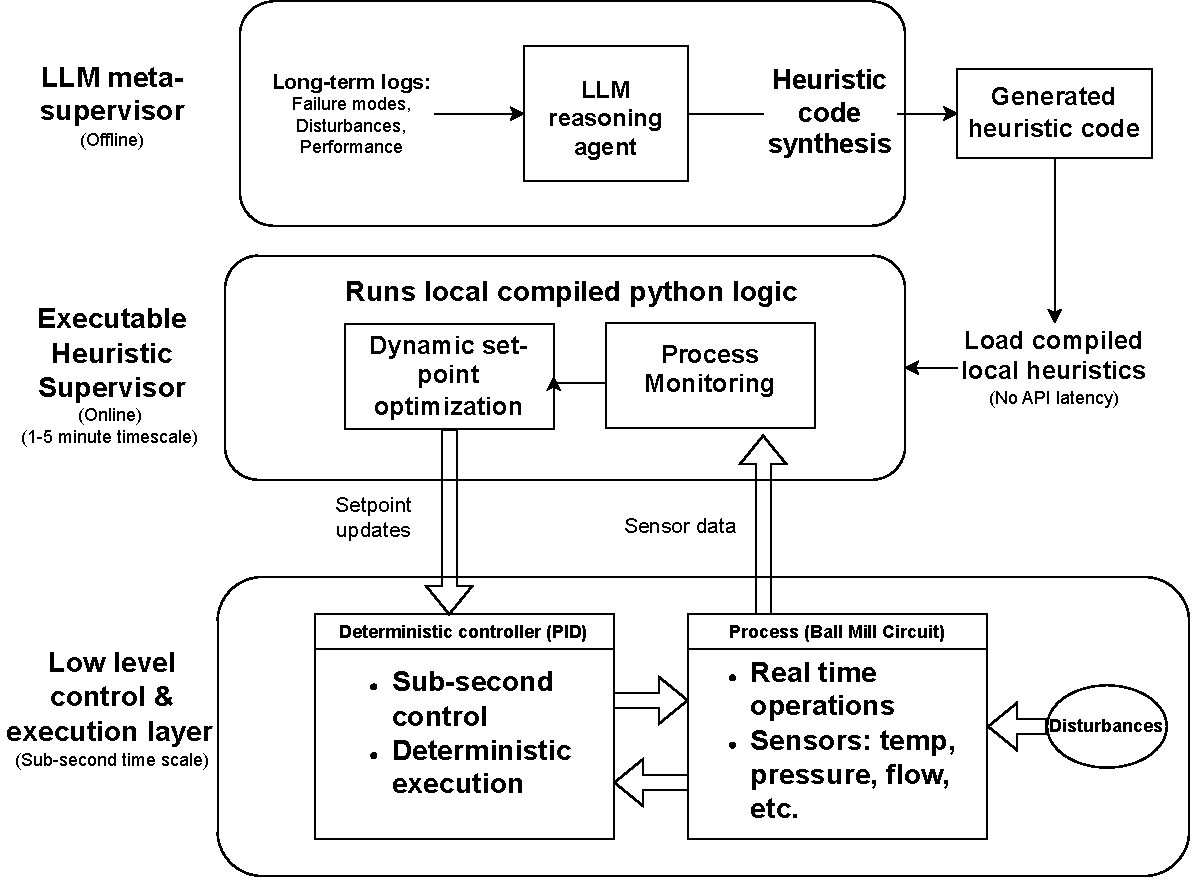
\includegraphics[width=\textwidth]{three_layer_architecture}
  \caption{The three-layer architecture, shown for the grinding circuit. The
    LLM meta-supervisor works offline on logged data and synthesizes
    heuristic code, which the executable supervisor runs locally without API
    calls. In the toy examples, the process is a tank simulation and the
    supervisor runs every 3--10~s.}
  \label{fig:architecture}
\end{figure}

\section{Supervisor interface}
Every supervisor implements the same function,
\begin{center}
\texttt{supervise(telemetry\_window, active\_setpoints, nominal\_targets)},
\end{center}
where the telemetry window holds, for each controlled tank and each sample,
the level, the output of the loop regulating it (pump effort) and the control
error. The function returns a free-text diagnosis, one adjusted setpoint per
loop (clamped to an allowed range) and one boolean anomaly flag per loop. It
is stateless: it is reloaded for every run and sees only its arguments.
The returned flags are held until the next decision. The setpoint-coordination
experiments in Chapter~\ref{ch:coord} use a variant of this interface
without anomaly flags.

\section{Security sandbox}
\label{sec:sandbox}
Generated code is treated as untrusted and passes three checks before it runs
on any telemetry:
\begin{enumerate}
\item a static check of the abstract syntax tree that rejects imports,
  \texttt{exec}, \texttt{eval}, file and network access, access to dunder
  attributes, oversized sources and anything other than a single top-level
  \texttt{supervise} function with the required signature;
\item execution in a namespace with an explicit whitelist of built-in
  functions and the \texttt{math} and \texttt{statistics} modules, instead of
  Python's real built-ins;
\item a wall-clock timeout on every call (0.5~s), so that an infinite loop
  cannot stall the simulation.
\end{enumerate}
An exception or timeout during evaluation is recorded as a failure, the
setpoints are held and both anomaly flags are raised.

\section{Evaluation and scoring}
\label{sec:scoring}
Each candidate is simulated in closed loop on a fixed \emph{development}
battery of fault scenarios: a fault-free run, single leaks of different onset,
size and duration, simultaneous leaks, persistent severe leaks and, for the
single- and two-tank processes, sensor noise. For a scenario $s$ the score is
\begin{equation}
  J_s = \mathrm{IAE}_s + 500\,V_s + 300\,M_s + c_{\mathrm{FP}}\,F_s
        + 10^4\,E_s + 200\,R_s ,
  \label{eq:score}
\end{equation}
where $\mathrm{IAE}_s$ is the integrated absolute tracking error of all
loops, $V_s$ the number of samples outside the safety bounds, $M_s$ and $F_s$
the number of samples, summed over loops, in which a held anomaly flag
disagrees with the true fault state (missed anomalies and false positives),
$E_s$ the number of exceptions and timeouts, and $R_s$ the distance between
the final and the nominal setpoints for loops whose fault has cleared. The
battery score $J$ is the average of $J_s$ over the scenarios; lower is
better.

Early candidates found several ways to improve $J$ while behaving worse,
which led to three safeguards:
\begin{itemize}
\item \emph{Asymmetric false-positive cost.} A false positive on a loop that
  never faults in the scenario costs $c_{\mathrm{FP}} = 800$ (250 on the
  quadruple-tank process); otherwise $c_{\mathrm{FP}} = 160$. Without this,
  flagging constantly was a cheap way to avoid missed anomalies.
\item \emph{Per-scenario regression guard.} A candidate is promoted only if it
  improves $J$ \emph{and} no single scenario gets worse than the champion by
  more than 5 points (fault-free scenario) or the larger of 100 points and
  15\% (fault scenarios). Averaging otherwise let a candidate win by breaking
  one scenario badly.
\item \emph{Held-out battery.} A second battery with the same scenario types
  but different fault timing and magnitude is never used for promotion. Its
  score is reported to the LLM only as a generalization gap.
\end{itemize}
For the quadruple-tank process an \emph{oracle} is also evaluated. It sets
each flag to the true fault state at every decision and keeps the nominal
setpoints, which is the best detection possible at the given decision
interval. It gives a lower bound that makes it possible to tell whether a
plateau is caused by the search or by the test bed.

\section{Training loop}
Each generation of the LLM meta-supervisor performs the following steps.
\begin{enumerate}
\item Build a prompt. The part that is the same in every call contains a
  description of the process at the level a plant engineer would know it
  (layout, mass balances, parameters, loop pairing, operating point and fault
  types), measured statistics of healthy operation, the calling contract, the
  exact list of allowed built-in functions, the scoring rules, the task and
  the output format. The part that changes contains the champion's source
  code, its per-scenario results, one line per decision for its two
  worst-scoring scenarios (true fault state against returned flags, errors,
  pump efforts and setpoints), a summary of the previous generation's
  rejected candidates, and a list of lessons learned.
\item Sample $K$ candidates from the LLM in parallel. Each response is a JSON
  object with a failure analysis, a numeric self-check of the thresholds
  against the healthy statistics, the new code and at most two new lessons
  of at most 30 words each.
\item Check, load and score every candidate, and promote the best one that
  passes the regression guard.
\end{enumerate}
The quadruple-tank experiments use DeepSeek's \texttt{deepseek-flash} model
through its API, with a configurable reasoning effort (none, low or high),
and the full loop with $K=4$. The loop was built up incrementally: the
single- and two-tank experiments used an earlier version with one candidate
per trial ($K=1$), aggregate failure counts instead of decision traces and
only a short qualitative description of the process, and they were run while
the setup was still changing, with more than one DeepSeek model.
An example of a generated supervisor is given in Appendix~\ref{app:supervisor}.
\TODO{State the prompt size (about 6\,500 tokens on the quadruple-tank process).}

\chapter{Toy examples}
\label{ch:toy}
The approach was developed on three simulated processes of increasing
difficulty, all with leaks as the fault type. Scores are comparable within a
process but not between processes, since the scenarios and weights differ.
Table~\ref{tab:summary} summarizes the results. All numbers in this chapter
are re-evaluated with the final scoring rules of each process.

\begin{table}[tb]
  \centering
  \caption{Average score $J$ (lower is better) with PID control only and with
    the best generated supervisor. For the quadruple-tank process the best
    supervisor equals the perfect-detection oracle.}
  \label{tab:summary}
  \begin{tabular}{@{}lrrrr@{}}
    \toprule
    & \multicolumn{2}{c}{Development} & \multicolumn{2}{c}{Held-out} \\
    \cmidrule(lr){2-3}\cmidrule(l){4-5}
    Process & PID only & Supervisor & PID only & Supervisor \\
    \midrule
    Single tank      & 31\,133 & 7\,551 & 30\,945 & 10\,487 \\
    Two-tank cascade & 30\,775 & 8\,720 & 35\,274 & 13\,744 \\
    Quadruple tank   & 64\,865 & 2\,635 & 69\,569 &  2\,609 \\
    \bottomrule
  \end{tabular}
\end{table}

\section{Single tank}
\label{sec:single}
\paragraph{Setup.} One tank with a pump controlled by a PID loop
($K_p = 2$, $K_i = 0.5$, $K_d = 0.1$) at a sample time of 0.1~s, and an
unmeasured leak as the fault. The supervisor decides every 3~s on the last
30 samples of a 30~s episode. The development battery has eight scenarios:
fault-free, a standard leak, an early severe leak, a late mild leak, two
leaks that start and stop, and a fault-free and a leaking scenario with
sensor noise. The held-out battery has the same types with other parameters.

\paragraph{Results.} Of 62 trials, 16 were promoted. The final supervisor
reduced the development score by 76\% and the held-out score by 66\%
compared with PID alone. Its remaining cost is dominated by false positives:
across the development battery it has 192 false-positive samples against 34
missed ones, and one of its decisions in the fault-free scenario is a false
alarm.

\paragraph{Findings.} Early supervisors lowered the setpoint during a fault
and never raised it again, which led to the restoration term $R_s$ in
\eqref{eq:score}; the false-positive weight was also tuned during this
example. The held-out score was 39\% worse than the development score, a
first sign that the search fits the timing of the visible scenarios.

\section{Two-tank cascade}
\label{sec:two}
\paragraph{Setup.} Tank~1 drains by gravity into tank~2, and each tank has
its own pump and PID loop with the same gains as above. A leak in tank~1
alone moves the level of tank~2 by more than 2~m, so the supervisor must tell
propagated disturbances from genuine faults. The development battery has
eight scenarios: fault-free, a leak in either tank, simultaneous leaks,
severe persistent leaks in either tank, and a fault-free and a leaking
scenario with sensor noise.

\paragraph{Results.} Of 58 trials, 7 were promoted and 10 were rejected by
the regression guard: each improved the average score while making one
scenario much worse. The final supervisor reduced the development score by
72\% and the held-out score by 61\%. The held-out score was 58\% worse than
the development score.

\paragraph{Findings.} This example exposed specification gaming: a candidate
improved the average score by flagging anomalies almost constantly. A false
positive cost the same in the fault-free scenario as anywhere else, and the
loss there was outweighed by fewer missed anomalies elsewhere. This led to the
asymmetric false-positive cost and the per-scenario regression guard in
Section~\ref{sec:scoring}. The most instructive lesson recorded by the LLM was
that the supervisor's own mitigation corrupted its detection statistic.
Lowering the setpoint of a leaking tank lowers the pump effort needed to hold
it, so an effort-based detector saw the fault disappear, cleared the flag,
restored the setpoint and then detected the fault again. The resulting
oscillation showed up as matched bursts of missed anomalies and false
positives in every single-fault scenario. The LLM removed it by normalizing
the pump effort with the tank's own level, which makes the statistic
insensitive to setpoint changes. It also learned to separate propagated from
genuine downstream faults with a residual test: the excess effort in tank~2
minus a coupling gain times the excess effort in tank~1. Simultaneous faults
remained unsolved: every candidate that improved them lost robustness to
sensor noise, and consecutive trials often repeated nearly identical
proposals.

\section{Quadruple-tank process}
\label{sec:four}
\paragraph{Setup.} The quadruple-tank process \cite{johansson2000} from the
PC-Gym benchmark suite \cite{bloor2024pcgym} has four tanks and two pumps.
Each pump feeds one lower tank directly and, through a split valve, the upper
tank above the other lower tank. With the split fractions
$\gamma_1 = \gamma_2 = 0.2$, most of each pump's flow takes the delayed path,
which gives a non-minimum-phase process. Only the two lower levels are
measured. The model is integrated with the explicit Euler method at a 1~s
step over 600~s episodes. A leak multiplies the outlet area of a lower tank
by 1.8--4. There are six development and six held-out scenarios, and the
supervisor decides every 10~s on the last 50~s of telemetry.

\subsection{A plateau caused by the test bed}
The first training runs stalled at $J \approx 36\,300$. Analysis showed
three defects in the test bed rather than a limit of the search:
\begin{enumerate}
\item \emph{Faults were never applied.} They were injected through PC-Gym's
  environment wrapper, which silently integrated an unmodified copy of the
  model, so the first twenty or so trials ran without any faults. The model
  is now integrated directly.
\item \emph{Decision interval.} The supervisor decided only every 50~s, the
  same as its window length, and every development fault started on that
  grid. Each fault event therefore cost at least 51 missed and 51
  false-positive samples, however good the detector was. With decisions
  every 10~s on the same 50~s window, the unchanged champion's score fell
  from 36\,300 to 26\,323.
\item \emph{Loop pairing.} The relative gain of the diagonal pairing is
  \begin{equation*}
    \lambda = \frac{\gamma_1\gamma_2}{\gamma_1+\gamma_2-1} = -0.07 ,
  \end{equation*}
  so the loops should be paired off-diagonally \cite{johansson2000}. With the
  diagonal pairing, a leak in tank~1 saturated pump~1, whose flow mostly
  reaches tank~2; loop~2 then reduced pump~2 and drained tank~3, which is
  tank~1's main supply. The resulting 171 safety violations in the severe
  tank-1 scenario made up 39\% of the average score, and a grid search showed
  that no setpoint policy could remove them. After re-pairing and retuning
  the loops as PI controllers ($K_p = 40$, $K_i = 0.3$), PID control alone
  gave no violations in any scenario.
\end{enumerate}
At the plateau, the champion was within about 7\% of the best score any
supervisor could reach on the flawed test bed. Computing such a bound before
interpreting a plateau would have revealed the problem much earlier.

\subsection{Results after the corrections}
Table~\ref{tab:four} shows the corrected test bed. The best supervisors flag
every leak at the first decision after it starts and clear the flag at the
first decision after it stops, which gives exactly the oracle's number of
missed and false-positive samples in all twelve scenarios. Three insights
appear in their code and lessons: the loop regulating a leaking tank
saturates at the 12~V pump limit, and this is the one signature that the
supervisor's own setpoint reduction cannot hide; a falling level together
with an error above the healthy maximum reveals a leak several seconds
before saturation; and the rate at which a level rises separates the slow
creep of a leaking tank from refilling after a leak has stopped.

\begin{table}[tb]
  \centering
  \caption{Quadruple-tank process after the test-bed corrections.}
  \label{tab:four}
  \begin{tabular}{@{}lrr@{}}
    \toprule
    Supervisor & Development & Held-out \\
    \midrule
    PID only (and the seed supervisor)          & 64\,865 & 69\,569 \\
    Plateau champion, not retrained             & 10\,777 & 14\,941 \\
    Best generated (low reasoning, generation 2) &  2\,635 &  2\,609 \\
    Perfect-detection oracle                    &  2\,635 &  2\,609 \\
    \bottomrule
  \end{tabular}
\end{table}

\subsection{Effect of LLM reasoning}
The same search was run from the seed supervisor with three reasoning
settings (Figure~\ref{fig:reasoning} and Table~\ref{tab:reasoning}). With
high and low reasoning the search matched the oracle on both batteries within
three and two generations, respectively, and the held-out scores followed the
development scores. Without reasoning the search improved quickly at first
but stalled at 11\,837 from the third generation on, about 4.5 times the
oracle score. Three weaknesses stood out without reasoning: it missed 49--83
samples in each scenario with a mild leak, against 4--12 with reasoning; its lessons contained
incorrect physics, for example that a leak lowers the other loop's effort
through a shared outflow path that does not exist; and three of twelve
candidates in generations 4--6 called a built-in function that the sandbox
does not provide, after the prompt's list of allowed functions ended in
``etc.''. The list is now generated from the sandbox itself. With high
reasoning, 8 of 15 requests returned an empty response that was still
billed.

\begin{figure}[tb]
  \centering
  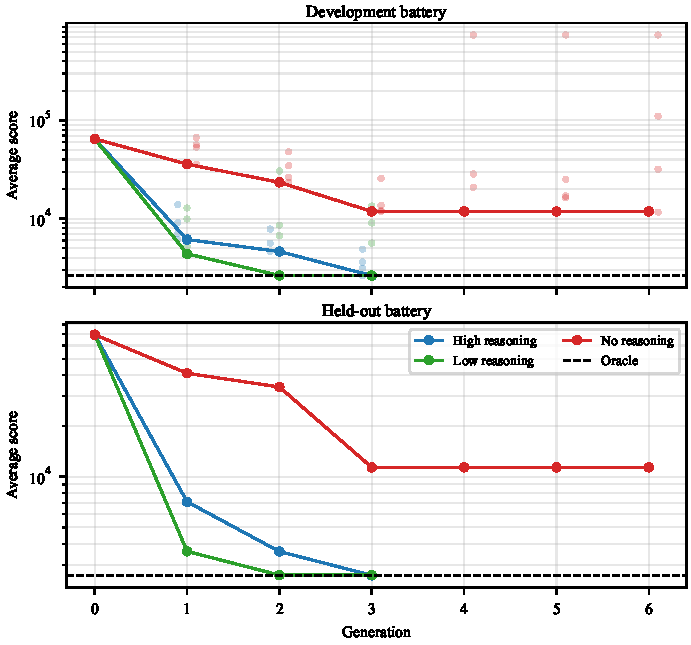
\includegraphics[width=\textwidth]{four_tank_reasoning_comparison}
  \caption{Score of the champion after each generation for three reasoning
    settings, on the development and held-out batteries (log scale). Dots
    are individual candidates; the three near $7\cdot 10^5$ crashed on every
    call. Generation~0 is the seed supervisor. The high-reasoning run used
    low reasoning in its third generation and an earlier, longer prompt in
    its first two.}
  \label{fig:reasoning}
\end{figure}

\begin{table}[tb]
  \centering
  \caption{Cost of reaching the oracle with different reasoning settings
    (DeepSeek off-peak prices, US dollars).}
  \label{tab:reasoning}
  \begin{tabular}{@{}lccc@{}}
    \toprule
    Reasoning & Generations & Output tokens & Cost \\
              & to oracle   & per request   & to oracle \\
    \midrule
    High & 3 & $\approx 61\,000$ & $\approx 0.63$ \\
    Low  & 2 & $\approx 23\,000$ & $\approx 0.11$ \\
    None & not reached in 6 & $\approx 2\,000$ & -- \\
    \bottomrule
  \end{tabular}
\end{table}

Each setting was run only once, and the runs differ slightly in their
prompts as noted in Figure~\ref{fig:reasoning}. The results therefore support
the conclusion that reasoning is needed and that low reasoning is enough for
this task, but not a precise ranking of low against high reasoning.
\TODO{Repeat each setting two or three times with the final prompt.}

\chapter{Discussion}
\label{ch:discussion}

\section{The evaluation matters as much as the model}
On all three processes, the largest improvements came from changes to the
evaluation, not to the model. The search exploited every weakness in the
score that it could find: constant flagging, breaking one scenario to win on
average, and fitting the timing of the visible scenarios. On the
quadruple-tank process, a long plateau turned out to be caused by the test
bed itself: faults that were never applied, a decision interval that fixed
a floor on the score, and a base-layer pairing that made one scenario
impossible. A perfect-detection oracle exposed the last two immediately
once it was computed. Checking that the test bed is sound, and bounding what
is achievable, should come before interpreting the progress of the search.

\section{What the LLM needs}
Progress on the quadruple-tank process was much faster after the prompt
gained a plant-engineer-level description of the process and per-decision
traces of the champion's worst scenarios. This agrees with AlphaEvolve and
Eureka, where removing problem context or result feedback degraded the
search \cite{novikov2025alphaevolve,ma2024eureka}. Sampling several
candidates per generation also mattered: the candidates of one generation
often differed in score by a factor of two or more.
\TODO{Quantify this with an ablation of the process description and the traces.}

\section{Reasoning}
Without reasoning, the LLM made steady early progress at about a
twenty-fifth of the cost, but then stalled, wrote physically incorrect
lessons and made avoidable coding mistakes. Because lessons are shown to
later generations as constraints, an incorrect lesson can keep steering the
search in the wrong direction. Low reasoning was enough to reach the oracle
and was about six times cheaper than high reasoning, which also produced
many empty, billed responses.

\section{Interpretability}
Every champion is a single Python function of 43 to 210 lines with named
thresholds and a diagnosis string for each decision. The supervisor that
matched the oracle on the quadruple-tank process
(Appendix~\ref{app:supervisor}) has 43 lines and flags a tank when any of
three conditions on the last 10~s holds: the level is falling while the error
is large; the loop's effort is above the healthy maximum while the error is
large and the level is not recovering; or the pump is close to saturation
and the level is not rising quickly. An engineer can read, test and modify
such a function, and the security sandbox guarantees that it cannot import
modules, touch files or run indefinitely. This is the main advantage over a
learned black-box controller.
\TODO{Discuss how interpretable the longer single- and two-tank supervisors are in practice.}

\section{Limitations}
\begin{itemize}
\item The processes are small simulations with a single fault type (leaks),
  and the quadruple-tank process has noise-free measurements.
\item Each configuration was trained once; the search is stochastic, so
  repeated runs are needed for firm conclusions.
\item The batteries are small (six to eight scenarios each), and the single-
  and two-tank supervisors generalized noticeably worse to the held-out
  scenarios.
\item The tracking error is measured against the active setpoint, so a
  supervisor can reduce it slightly by lowering the setpoint of a leaking
  tank without improving the process. On the quadruple-tank process this is
  worth about 10 points per scenario.
\item No comparison with TD-MPC or any other learned controller has been made
  yet.
\end{itemize}

\chapter{Conclusions and future work}
\label{ch:conclusions}

\section{Conclusions}
An LLM used offline as a meta-supervisor produced deterministic,
security-checked supervisors that reduced the development score by
72--96\% compared with PID control alone on three toy processes. On the
quadruple-tank process, the generated supervisor matched a perfect-detection
oracle on both development and held-out scenarios within two generations,
with low reasoning effort and at a cost of about 0.11 US dollars. Reaching
this required a sound test bed and a score protected against specification
gaming, and it required some LLM reasoning: without it the search stalled
well above the oracle.

On a setpoint-coordination version of the quadruple-tank process, which
rehearses the industrial comparison, the best generated supervisor came
within 1.3\% of a model predictive controller with online disturbance
estimation on the development scenarios, and was 11\% worse on held-out
scenarios and 6.7\% worse beyond the development range. Like the MPC it
degraded sharply beyond the development range, but it gave up constraint
satisfaction to hold production, where the MPC did the opposite. Reaching
this score took a regression guard that loosens in early generations, a
measured record of failed changes in the prompt and high reasoning effort,
and it was reached in a single run; all coordination runs together cost
about 4 US dollars.
\TODO{Answer the research questions once the industrial study is done.}

\section{Future work}
\begin{itemize}
\item Apply the method to the industrial process and data at Weir and
  compare it with the TD-MPC controller in use there.
\item Make the toy benchmark harder: sensor noise and model mismatch on the
  quadruple-tank process, other fault types such as pump wear and sensor
  drift, and tracking error measured against the nominal setpoint.
\item Repeat each configuration several times, and ablate the process
  description and the decision traces. For setpoint coordination, separate
  the effect of high reasoning effort from that of the inherited record of
  failed changes.
\item Fix the weights of the coordination score with Weir's operators
  before the industrial comparison.
\end{itemize}


\printbibliography

\appendix
\chapter{Example of a generated supervisor}
\label{app:supervisor}
The listing below is the complete supervisor generated in the second
generation of the low-reasoning run on the quadruple-tank process
(Section~\ref{sec:four}). It matches the perfect-detection oracle on both
the development and the held-out battery. Line breaks inside parentheses
were added to fit the page; the code is otherwise unchanged.

{\footnotesize
\begin{verbatim}
def supervise(telemetry_window, active_setpoints, nominal_targets):
    DROP_SLOPE = -0.0015
    DROP_ERR = 0.03
    DROP_MARGIN = 0.02
    EFF_HI = {'tank1': 10.7, 'tank2': 10.0}
    EFF_ERR = 0.05
    RECOV_SLOPE = 0.0003
    SAT_EFF = 11.8
    SAT_RECOV = 0.0015

    def eval_tank(tank):
        sp = float(nominal_targets[tank])
        levels = [s[tank]['level'] for s in telemetry_window]
        efforts = [s[tank]['pump_effort'] for s in telemetry_window]
        n = len(levels)
        if n == 0:
            return False
        L = levels[-1]
        err = sp - L
        k = min(10, n)
        if k > 1:
            slope10 = (levels[-1] - levels[-k]) / float(k - 1)
        else:
            slope10 = 0.0
        if n >= 10:
            e_max10 = max(efforts[-10:])
        else:
            e_max10 = max(efforts)
        drop = ((slope10 < DROP_SLOPE) and (err > DROP_ERR)
                and (L < sp - DROP_MARGIN))
        effort_flag = ((e_max10 >= EFF_HI[tank]) and (err > EFF_ERR)
                       and (slope10 <= RECOV_SLOPE))
        sat = (e_max10 >= SAT_EFF) and (slope10 < SAT_RECOV)
        return bool(drop or effort_flag or sat)

    a1 = eval_tank('tank1')
    a2 = eval_tank('tank2')

    return {
        'diagnosis': ('tank1 anomaly=' + str(a1)
                      + '; tank2 anomaly=' + str(a2)),
        'adjusted_setpoints': {
            'tank1': float(nominal_targets['tank1']),
            'tank2': float(nominal_targets['tank2']),
        },
        'anomaly_flags': {'tank1': bool(a1), 'tank2': bool(a2)},
    }
\end{verbatim}
}

\end{document}
